\resizebox{0.25\textwidth}{!}{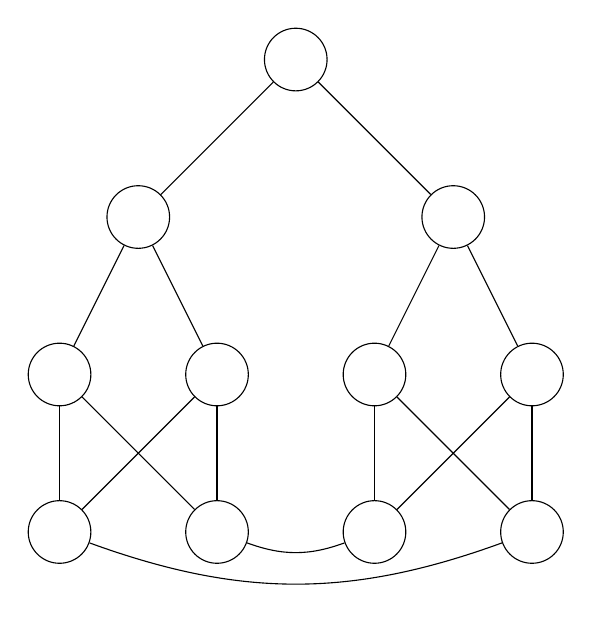
\begin{tikzpicture}[myv/.style={circle, draw, inner sep=8pt},myv1/.style={circle, draw, inner sep=0pt,color=white},myv2/.style={rectangle, draw,dotted,inner sep=0pt,line width = 0.5mm}]
 % \node [label=above: $\Large{r}$](z)  at (0,4) {};

  \node[myv] (a) at (0,4) {};
  \node[myv] (b) at (-2,2) {};
  \node[myv] (c) at (2,2) {};

  \node[myv] (d) at (-3,0) {};
  \node[myv] (e) at (-1,0) {};
  \node[myv] (f) at (1,0) {};
  \node[myv] (g) at (3,0) {};

  \node[myv] (h) at (-3,-2) {};
  \node[myv] (i) at (-1,-2) {};
  \node[myv] (j) at (1,-2) {};
  \node[myv] (k) at (3,-2) {};
   \node[myv1] (l)  at (3,-2.5) {};
   \node[myv1] (m)  at (3,-3) {};
  
    \draw (a) -- (b);
    \draw (a) -- (c);
    \draw (b) -- (d);
    \draw (b) -- (e);
    \draw (c) -- (f);
    \draw (c) -- (g);
    \draw (d) -- (h);
    \draw (d) -- (i);
    \draw (e) -- (h);
    \draw (e) -- (i);
    \draw (f) -- (j);
    \draw (f) -- (k);
    \draw (g) -- (j);
    \draw (g) -- (k);
    \draw (i) to [bend right=20] (j);
    \draw (h) to [bend right=20] (k);

   

\end{tikzpicture}}
